\documentclass{beamer}

\usepackage[utf8]{inputenc}
%\usepackage{beamerthemesplit}
\usepackage{url}
\usepackage{tikz}
\usepackage{alltt}
\usepackage{listings}
\usepackage{marvosym}
\usepackage{color}
\usepackage[multidot]{grffile}
\usepackage{multirow}
\usepackage{array}
\usepackage{setspace}
\usepackage{hyperref}
\usepackage{verbatim}
\usepackage{fancyvrb}
%\hypersetup{colorlinks=true, linkcolor=blue,  anchorcolor=blue,  
%citecolor=blue, filecolor=blue, menucolor=blue, pagecolor=blue,  
%urlcolor=blue} 
\lstset{keywordstyle=\bfseries\color{brown},
        stringstyle=\ttfamily,
        commentstyle=\color{blue}\textit,
        showstringspaces=false}

\useoutertheme{}
\usetheme{Madrid}
\graphicspath{{pics/}{global/}
{pics/I/}{pics/A1/}{pics/A2/}{pics/A3/}{pics/A4/}{pics/A5/}{pics/A6/}{pics/A7/}
}

\logo{
\includegraphics[height=1cm]{ProcessHorizontal}} 

\institute{Center for Computation and Technology\\Louisiana State University, Baton Rouge, LA}

\setbeamertemplate{navigation symbols}{} 

\title{CSC 7700: Scientific Computing}

% We want to use the infolines outer theme because it does not use a lot of
% space, but it also tries to print an institution and the slide
% numbers (which we might not want to show). Therefore, we here redefine the
% footline ourselfes - mostly a copy & paste from
% /usr/share/texmf/tex/latex/beamer/themes/outer/beamerouterthemeinfolines.sty
\defbeamertemplate*{footline}{infolines theme without institution and slide numbers}
{
  \leavevmode%
  \hbox{%
  \begin{beamercolorbox}[wd=.25\paperwidth,ht=2.25ex,dp=1ex,center]{author in head/foot}%
    \usebeamerfont{author in head/foot}\insertshortauthor
  \end{beamercolorbox}%
  \begin{beamercolorbox}[wd=.5\paperwidth,ht=2.25ex,dp=1ex,center]{title in head/foot}%
    \usebeamerfont{title in head/foot}\insertshorttitle
  \end{beamercolorbox}%
  \begin{beamercolorbox}[wd=.25\paperwidth,ht=2.25ex,dp=1ex,center]{date in head/foot}%
    \usebeamerfont{date in head/foot}\insertshortdate{}
  \end{beamercolorbox}}%
  \vskip0pt%
}

% Some useful commands
\newcommand{\abspic}[4]
 {\vspace{ #2\paperheight}\hspace{ #3\paperwidth}\includegraphics[height=#4\paperheight]{#1}\\
  \vspace{-#2\paperheight}\vspace{-#4\paperheight}\vspace{-0.0038\paperheight}}

\newcommand{\picw}[4]{{
 \usebackgroundtemplate{
 \color{black}\vrule width\paperwidth height\paperheight\hspace{-\paperwidth}\hspace{-0.01\paperwidth}
 \hspace{#4\paperwidth}\includegraphics[width=#3\paperwidth, height=\paperheight]{#1}}\logo{}
 \frame[plain]{\frametitle{#2}}
}}
\newcommand{\pic}[2]{\picw{#1}{#2}{}{0}}

\newcommand{\question}[1]{\frame{\frametitle{#1}
 \begin{centering}\Huge #1\\\end{centering}
}}



%\usecolortheme[RGB={200,200,200}]{structure}

\subtitle[Introduction]{\large Course Introduction}
\author[\mbox{
\includegraphics[height=0.6em]{fl_300}\hspace{0.5em}Frank Löffler}]{Dr Frank Löffler}
\date{August 30 2013}
\usecolortheme[RGB={90,90,90}]{structure}

\begin{document}

\frame{\titlepage}

\frame[containsverbatim]{ \frametitle{Our Goals}
 \begin{itemize}
  \item Building the experience and confidence that
        will encourage \textbf{you} to seek out and use national
        cyberinfrastructure and scientific computing techniques\\
        \textit{Make you not shy away from large computers}
  \item Demonstrating best practices of using and extending research software\\
        \textit{Make you not shy away from programming in teams}
  \item Showing how to efficiently collaborate with colleagues both locally
        and remote\\
        \textit{Make you not shy away from working in distributed teams}
 \end{itemize}
}

\frame{\frametitle{Course Information}
\begin{itemize}
 \item Class time: Fridays 8:20am-11:20am
 \item Class location
  \begin{itemize}
   \item Today: Tureaud Hall, Room 0101
   \item Later: LDMC (announced on class email list)
  \end{itemize}
 \item Email list for class: sci-comp-2013-class@mail.cct.lsu.edu
 \item Email list instructors: sci-comp-2013-instructors@mail.cct.lsu.edu
 \item Class web page:
%       {\small\url{https://wiki.cct.lsu.edu/sci-comp-2013/}}
        {\small\url{https://wiki.cct.lsu.edu/sci-comp/Main_Page}}
 \item Materials Subversion repository: 
       {\small\url{https://svn.cct.lsu.edu/repos/courses/sci-comp-2013/public}}
\end{itemize}
}

\frame{\frametitle{Course Organization}
 \begin{itemize}
  \item 5 overall topics
  \item 5 instructors
  \item 2-3 classes (Fridays) each instructor
  \item topics:
  \begin{itemize}
   \item A: Basic Skills
   \item B: Advanced Programming Tools
   \item C: Parallel Computing
   \item D: Simulations and Application Frameworks
   \item E: Distributed Scientific Computing
  \end{itemize}
 \end{itemize}
}

\frame{\frametitle{Dr Frank Löffler}
{\centering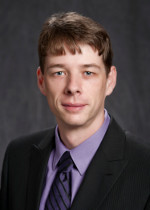
\includegraphics[height=3cm]{frank}\\}
\begin{itemize}
 \item Module A: Basic Skills
 \item Staff position at Center for Computation and Technology (CCT)
 \item Relativistic Astrophysics
 \item High-Performance Computing
\end{itemize}
}

\frame{\frametitle{Basic Skills - Motivation}
Challenge with ``incoming'' graduate students into research groups:
\begin{itemize}
 \item Wide variability in basic computer and computational skills and experience
 \item Unless students had already been partially trained in other research groups:
  \begin{itemize}
   \item Rarely have previous experience with HPC
   \item Would not know about the existence of, or the use of local, state-wide or
         national computing resources
   \item Rarely worked in large, distributed teams
   \item Often didn't work on large software projects yet
  \end{itemize}
\end{itemize}
}

\frame{\frametitle{Basic Skills}
\abspic{xsede-black}{0.23}{0.6}{0.1}
\begin{enumerate}
 \item Survival skills for Unix environments
 \item Revision control systems; Collaboration / project management
 \item Simple data visualization
 \item Three-dimensional data visualization
\end{enumerate}
}

\frame{\frametitle{Prof Steven Brandt}
{\centering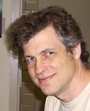
\includegraphics[height=3cm]{sbrandt}\\}
\begin{itemize}
 \item Module B: Advanced Programming Tools
 \item Faculty at CCT, Computer Science
 \item Software development specialist
 \item HPC expert
\end{itemize}
}

\frame{\frametitle{Advanced Programming Tools}
\begin{itemize}
 \item Compiling
 \item Debugging
 \item Profiling
 \item Programming (best) practices
 \item Accelerator computing
\end{itemize}
}

\frame{\frametitle{Prof Hartmut Kaiser}
{\centering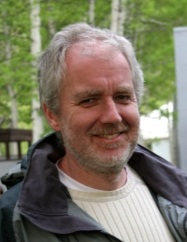
\includegraphics[height=3cm]{hartmut}\\}
\begin{itemize}
 \item Module C: Parallel Computing
 \item Assistant Professor at CCT, Computer Science
 \item Parallel programming and HPC expert
 \item C++ ``guru''
\end{itemize}
}

\frame{\frametitle{Parallel Computing}
\begin{itemize}
 \item The future of computing: going parallel
  \begin{itemize}
   \item MPI
   \item OpenMP
   \item other choices
  \end{itemize}
 \item Challenges in parallel computing
  \begin{itemize}
   \item typical bottlenecks
   \item possible (future) solutions
  \end{itemize}
\end{itemize}
}

\frame{\frametitle{Prof Peter Diener}
{\centering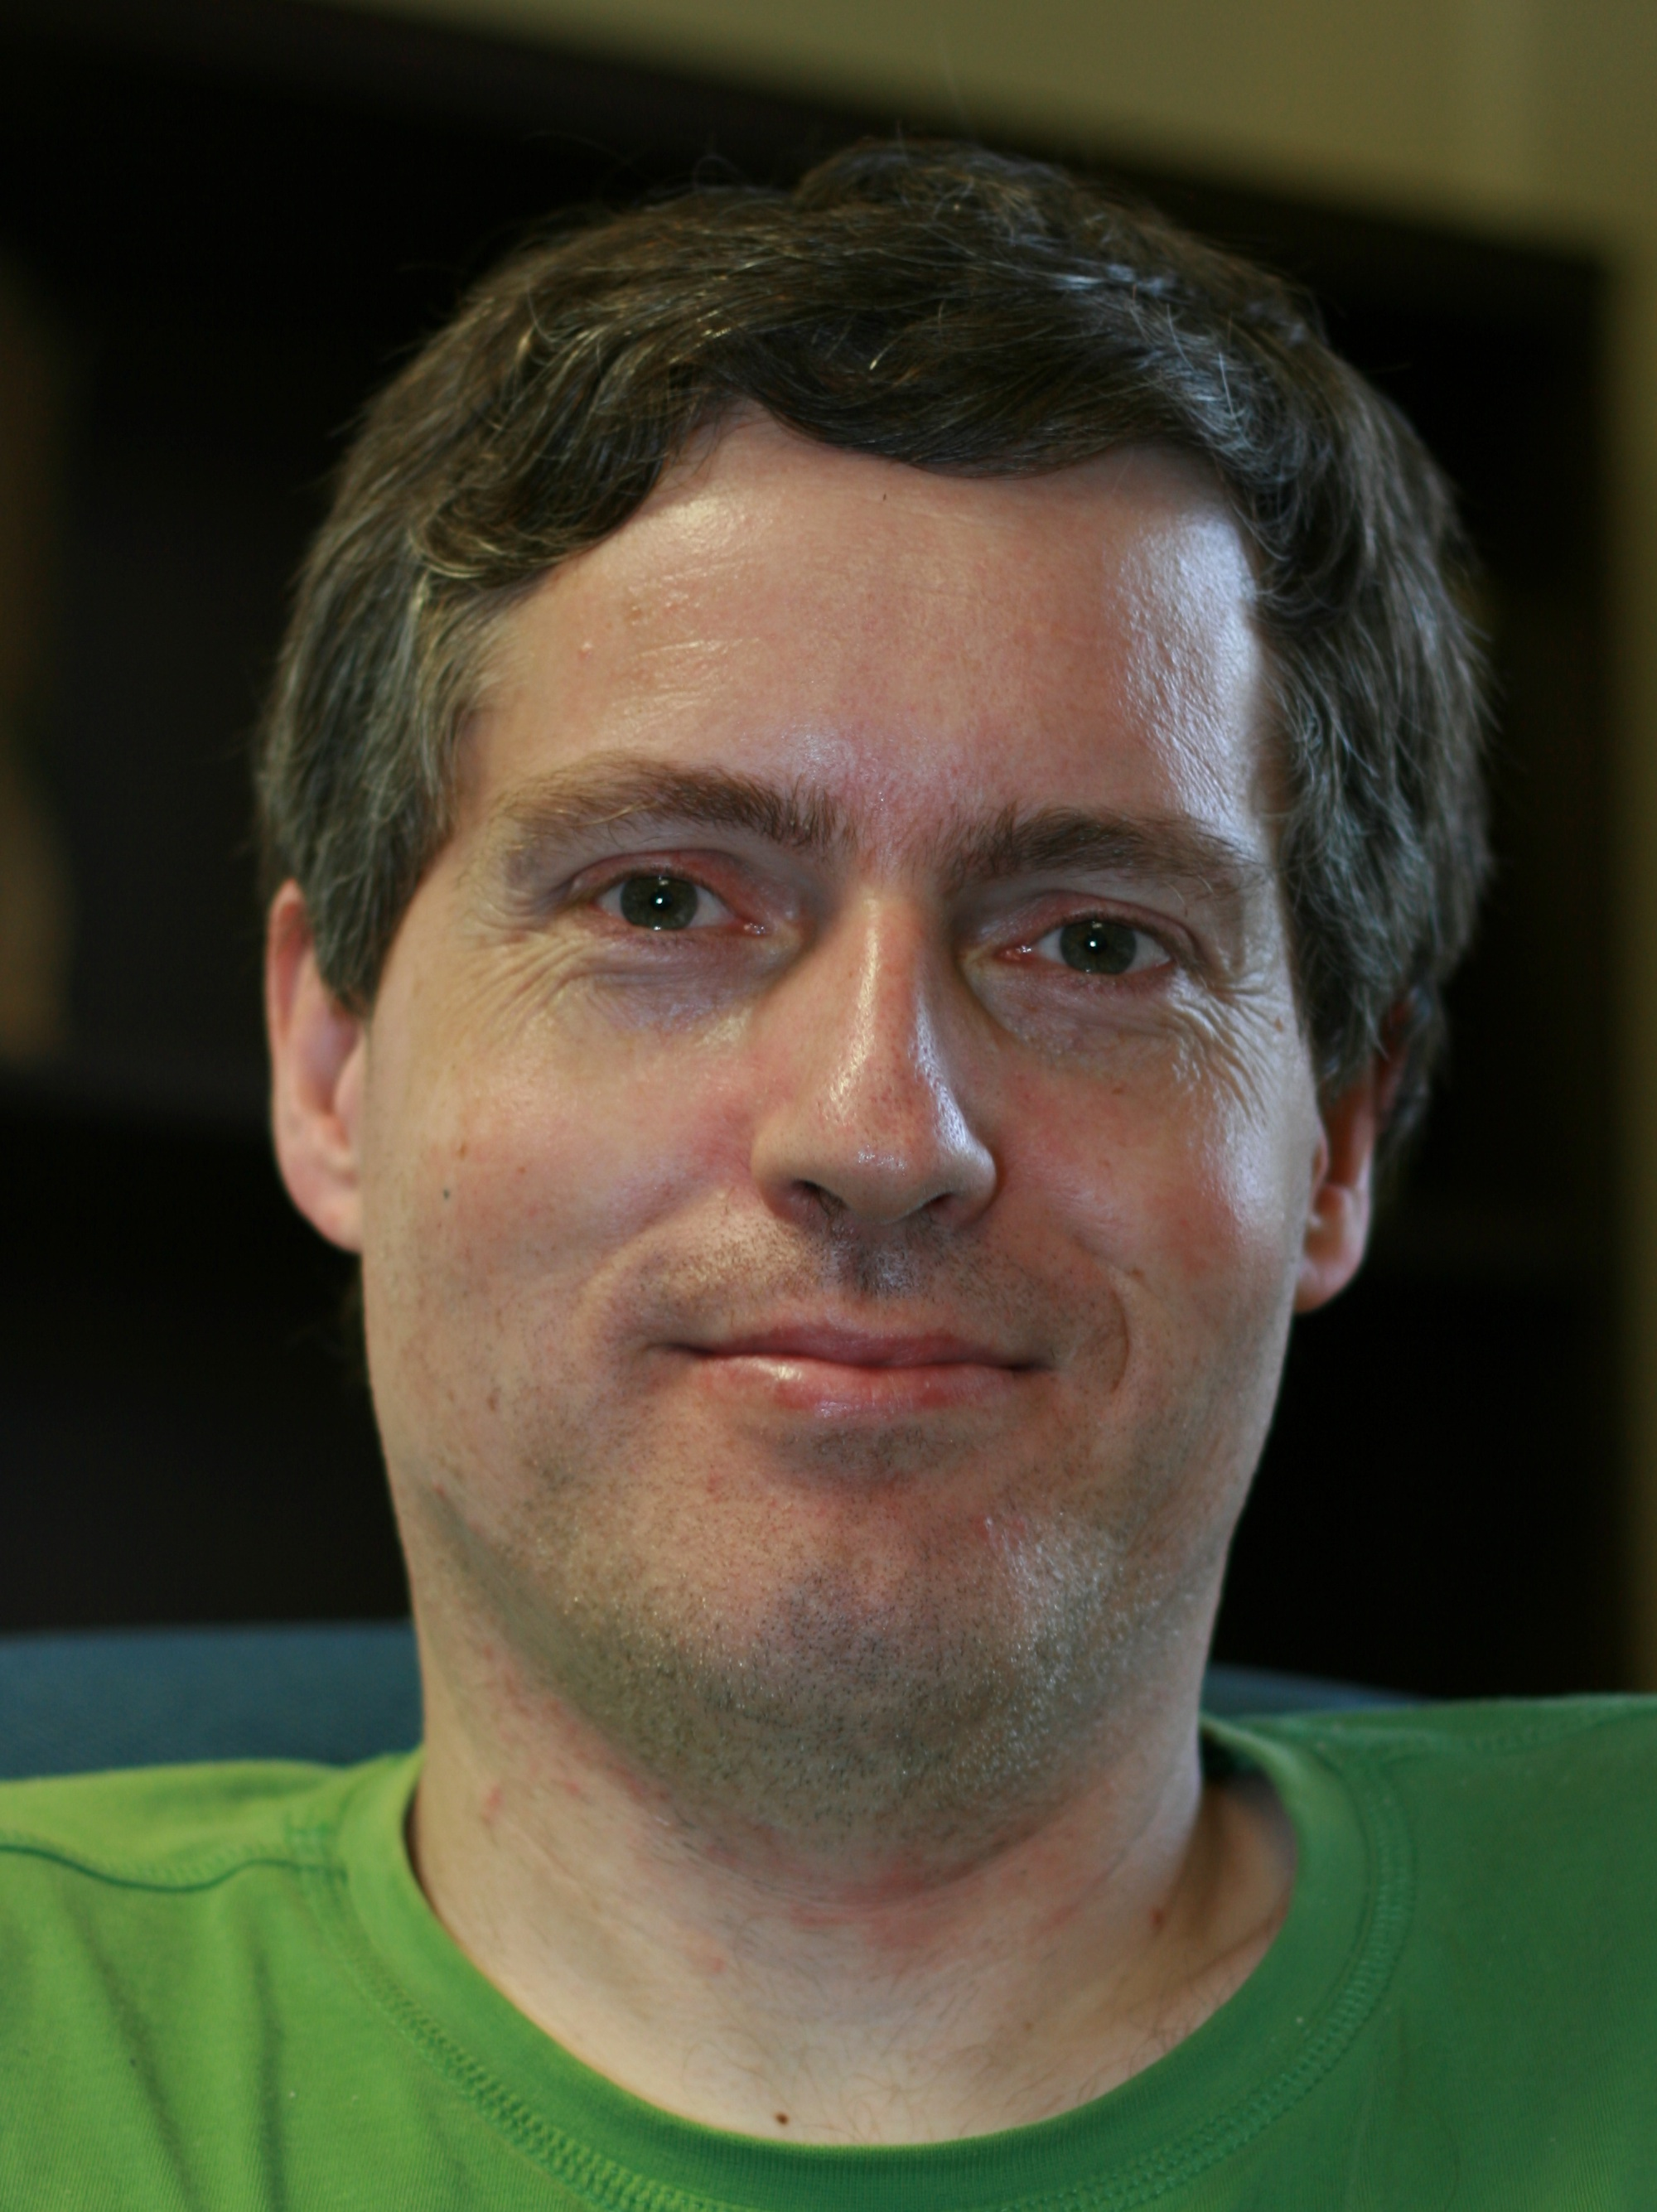
\includegraphics[height=3cm]{diener}\\}
\begin{itemize}
 \item Module D: Simulations and Application Frameworks
 \item Assistant Professor at CCT
 \item Relativistic Astrophysics
 \item High-Performance Computing
\end{itemize}
}

\frame{\frametitle{Simulations and Application Frameworks}
\abspic{BH_simulation}{0.11}{0.6}{0.2}
\abspic{kraken}{0.4}{0.55}{0.2}
Aim: explain the essential elements of modern simulation codes that are run on
     parallel supercomputers, especially Xsede systems.\\*[1em]Examples at LSU:
\begin{itemize}
 \item modeling black holes
 \item predicting the effects of hurricanes
 \item optimizing oil and gas production from underground reservoirs
\end{itemize}
\vspace{1em}Often not understood by students:
\begin{itemize}
 \item typical code structure
 \item scientific goals and needs
 \item hardware and technology limitations
\end{itemize}
}

\frame{\frametitle{Prof Shantenu Jha}
{\centering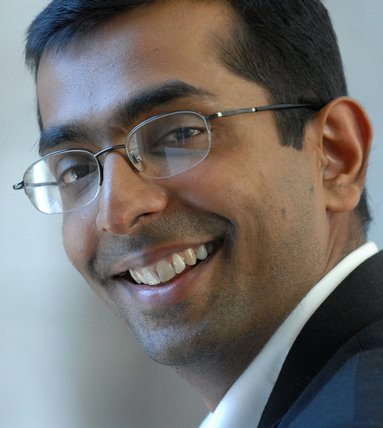
\includegraphics[height=3cm]{shantenu}\\}
\begin{itemize}
 \item Module E: Distributed Scientific Computing
 \item Assistant Professor, ECE, Rutgers University
 \item Former director of Cyberinfrastructure Development at CCT
 \item Distributed computing expert
\end{itemize}
}

\frame{\frametitle{Distributed Scientific Computing}
\abspic{cloud_computing}{0.1}{0.7}{0.15}
\begin{itemize}
 \item Introduction to the Practice of Distributed Computing
  \begin{itemize}
   \item Definition and application examples
   \item Comparison to HPC
  \end{itemize}
 \item Introduction to SAGA
 \item Examples of ``production'' grid infrastructure
 \item Building own distributed applications
 \item Introduction to Cloud computing
  \begin{itemize}
   \item Commercial/Enterprise Clouds
   \item FutureGrid
  \end{itemize}
 \item When to compute distributed and when rather not
\end{itemize}
}

\frame{\frametitle{Grading}
 \begin{itemize}
  \item Emphasis on practical work and experience
  \item No aim at tricky exam questions: convince with your experience
  \item Don't leave coursework until the last moment: it does \textbf{not} work here
  \item Course work of each module counts.
  \item No midterm, but review session
  \item Final Exam will be oral and will cover all modules.
 \end{itemize}
 \centering
 \begin{tabular}{l|l}
  Module A course work& 15\%\\
  Module B course work& 15\%\\
  Module C course work& 15\%\\
  Module D course work& 15\%\\
  Module E course work& 15\%\\
  Final Exam          & 25\%\\
 \end{tabular}\\
}

\frame{\frametitle{Famous Last (First) Words}
\begin{itemize}
 \item This class is for \textbf{YOU}
 \item Ask questions
 \item Give suggestions
 \item Do course work \textbf{early}
 \item Let us know of problems right away
\end{itemize}
}

\section*{Course Work}

\frame{\frametitle{Course Work: some general remarks}
 \begin{itemize}
  \item Do it early!
  \item Course work will form 75\% of your grade!
  \item If you have problems: contact us. This will not lower your grade.
        The only change it might have on your grade is positive.
  \item To be submitted electronically (see below)
  \item Deadlines are strict (end of the deadline day)
 \end{itemize}
}

\frame{\frametitle{Course Work: some general remarks}
 \begin{itemize}
  \item If not asked otherwise, submit reports in pdf, as single file.
        Other formats will not be accepted.
  \item If you are asked to write a program, submit the source code (text file,
        no pdf here) and, if
        applicable, a makefile - not the executable
  \item Make the reports look nice. This is (also) an exercise in report/paper writing.
  \item Include your name, the class number (CSC 7700) and a date.
  \item If you have graphs or pictures, include them in the pdf file. Don't submit
        separate files unless asked for.
 \end{itemize}
}

\frame[containsverbatim]{ \frametitle{Course Work A1}
 No pdf reports yet, but:\\
 \vspace{1em}
 \verb|https://portal.xsede.org/|
 \begin{itemize}
  \item Create Account
  \item Submit all necessary information and verify account
  \item \textbf{ASAP}!
  \item Send us email with your Xsede user name to\\
        sci-comp-2013-instructors@mail.cct.lsu.edu
 \end{itemize}
 \vspace{1em}
 \verb|https://accounts.hpc.lsu.edu/login_request.php|
 \begin{itemize}
  \item Request login
  \item Submit all necessary information and verify account
  \item LSU contact: Frank Löffler (Center for Computation and Technology)
  \item \textbf{ASAP}!
  \item Send us email with HPC user name to\\
        sci-comp-2013-instructors@mail.cct.lsu.edu
 \end{itemize}
}

\end{document}

